\documentclass[parskip=full]{scrreprt}

\usepackage[english]{babel}
\usepackage[utf8]{inputenc}
\usepackage{csquotes}
\usepackage[backend=biber]{biblatex}
\addbibresource{mainreport.bib}

\usepackage{graphicx}
  \graphicspath{ {./graphics/} }
\usepackage{url}
\usepackage{varioref}
\usepackage{tabularx}
  \newcolumntype{L}{>{\raggedright\arraybackslash}X}
  \usepackage[version=4]{mhchem}
\usepackage{siunitx}
\usepackage{booktabs}
\usepackage{longtable}

\author{Arin Wongprommoon\thanks{\texttt{aw729@cam.ac.uk}} \\University of Cambridge}
\title{Optimising production of citramalate based on the \emph{E. coli} kinetic model}
\subtitle{Project Report}
\date{17 August 2018}

\begin{document}

\maketitle

\tableofcontents

\begin{abstract}
  Using living organisms to synthesise chemicals is an alternative to synthesising chemicals from fossil fuels, as it serves as a renewable resource with potentially high efficiency and low cost. The procedures can be sped up by optimising conditions using mathematical models. Citramalate ((2S)-2-Hydroxy-2-methylbutanedioate) is a chemical of industrial interest as it can be a precursor for methacrylic acid, a monomer for the production of plastics. 
  
  The project aimed to find conditions to maximise the production of citramalate using modelling approaches. In this project, an existing kinetic model for \emph{E. coli} metabolism was extended by adding a reaction that produces citramalate from acetyl coenzyme A and pyruvate. \emph{E. coli} was chosen as the model organism as its metabolism is very well characterised in the literature. The project employed Python and libraries specific to genetic algorithms, modelling, and manipulating information presented in SBML (systems biology markup language).
  
  First, the effect of $V_{max}$ values of enzymes in the kinetic model~\cite{millard_metabolic_2017} on productivity of citramalate was investigated. $V_{max}$ values were chosen as a parameter as it can be easily tested \emph{in vivo} by relying on the principle that $V_{max}$ is proportional to enzyme concentration. The differential evolution genetic algorthim was then employed to compute the set of $V_{max}$ values of enzymes that optimises the production of citramalate, assuming Michaelis-Menten kinetics.
  
  In the second part of the project, information from the kinetic model was used to enrich the stoichiometric model~\cite{orth_comprehensive_2011}. More specifically, information about the possible values of fluxes through each reaciton was used to set the boundaries for each reaction in a stoichiometric model. Flux balance analysis (FBA) was then performed to evaluate the highest possible flux through the citramalate-producing reaction as a proxy for citramalate productivity. The composition of the Lund medium~\cite{eastham_process_2015} was studied in an attempt to create boundaries for relevant uptake reactions.
  
  The project took place at the Cambridge Systems Biology Centre, Department of Biochemistry, in Prof Steve Oliver's group. Research associate Dr Jorge J\'ulvez supervised me throughout the project. The project was entirely computational, and ran from 25 June 2018 to 17 August 2018.
\end{abstract}

\chapter*{Introduction}
\label{ch:intro}

The project concerns two models of \emph{E. coli} metabolism: a kinetic model described by Millard \emph{et al} in 2017~\cite{millard_metabolic_2017} and a stoichiometric model described by Orth \emph{et al} in 2011~\cite{orth_comprehensive_2011}. The kinetic model concerns a smaller set of reactions than the stoichiometric model, but it contains information about initial conditions (substrate concentrations and flux through reactions) which the stoichiometric model lacks.

The kinetic model contains 68 reactions, 49 of which include $V_{max}$ as a parameter. Of these, 41\footnote{ACEA, ACEB, ACK, ACN\_1, ACN\_2, ACS, ATP\_syn, CITRA\_SYN, CYTBO, EDA, EDD, ENO, FBA, FBP, FUMA, GDH, GLT, GND, GPM, LPD, MAD, MDH, MQO, PCK, PDH, PFK, PGI, PGK, PGL, PIT, PPC, PPS, PTA, PYK, RPE, RPI, SDH, SK, SQR, TPI, and ZWF} correspond to real enzyme-catalyzed reactions in \emph{E. coli}. To investigate citramalate production, a 69th reaction called CITRA\_SYN was added to the model. It models the reaction:

\begin{center}
  acetyl-CoA + pyruvate + \ce{H2O} $\rightarrow$ CoA-SH + \ce{H^+} + citramalate
\end{center}

with the kinetic law

\[
  \frac{\mathrm{d}[citramalate]}{\mathrm{d}t} = 
  \frac{V_{max} \cdot [acetyl-CoA]}{[acetyl-CoA] + K_{m}}
\]

assuming pyruvate is saturating. The $V_{max}$ is set to 4 mM s\textsuperscript{-1} and $K_{m}$ to 0.495 mM in the modified model.

Citramalate productivity is defined as $\mu Y_{P/S}$, where $\mu$ is the growth rate in reciprocal time units (h\textsuperscript{-1} in this project) and $Y_{P/S}$ is defined as mass of product over mass of substrate, which is glucose in this context. Manipulating the SBML file required the Python library \texttt{libsbml} and running simulations employed the \texttt{roadrunner} module. Throughout the project, the simulations were from 0 to 7,200 seconds, at which steady-state is attained for almost all the conditions (also see section~\vref{sec:couples}) %change this to a subsection investigating steady-state later

The stoichiometric model contains 2,584 reactions, and I have mapped 57 of them to their equivalents in the kinetic model (more details in section~\vref{sec:mapping}). By default, most of these reactions are unbounded (Orth \emph{et al}~\cite{orth_comprehensive_2011} provided details about this). In a similar vein to the kinetic model, a 2,585th reaction for citramalate production was added to the stoichiometric model using the COBRA module in Python. However, no kinetic parameters were added, as stoichiometric models do not contain this information. In addition to the citramalate synthesis reaction, a sink reaction to allow citramalate to leave the system was also added.

\chapter{Investigating the kinetic model}
\label{ch:kinetic}

%(Maybe write the purpose of doing this here? But I think the abstract and the introduction suffice)

\section{Varying $V_{max}$ values of one reaction at a time}
\label{sec:onereac}

Here I investigated the relationship between the value of $V_{max}$ of each reaction in the kinetic model and the resulting citramalate productivity at steady state -- i.e.\ after two hours. I varied the $V_{max}$ values of each of the 49 reactions\footnote{ACEA, ACEB, ACK, ACN\_1, ACN\_2, ACS, ATP\_MAINTENANCE, ATP\_syn, CITRA\_SYN, CYTBO, EDA, EDD, ENO, FBA, FBP, FUMA, GDH, GLT, GND, GPM, GROWTH, LPD, MAD, MDH, MQO, NADH\_req, NDHII, PCK, PDH, PFK, PGI, PGK, PGL, PIT, PPC, PPS, PTA, PYK, RPE, RPI, SDH, SK, SQR, TPI, XCH\_ACE1, XCH\_ACE2, XCH\_GLC, XCH\_ZWF} in the kinetic model that include $V_{max}$ as a parameter. The ranges 0.1--1.0 $V_{max}$ and 0.1--10.0 $V_{max}$, where $V_{max}$ is the wild-type $V_{max}$ for that particular reaction as specified in the SBML file. I used 100 data points for each plot. Figure~\ref{fig:onereacsample} is an example of such a plot.

\begin{figure}[htbp]
  \centering
  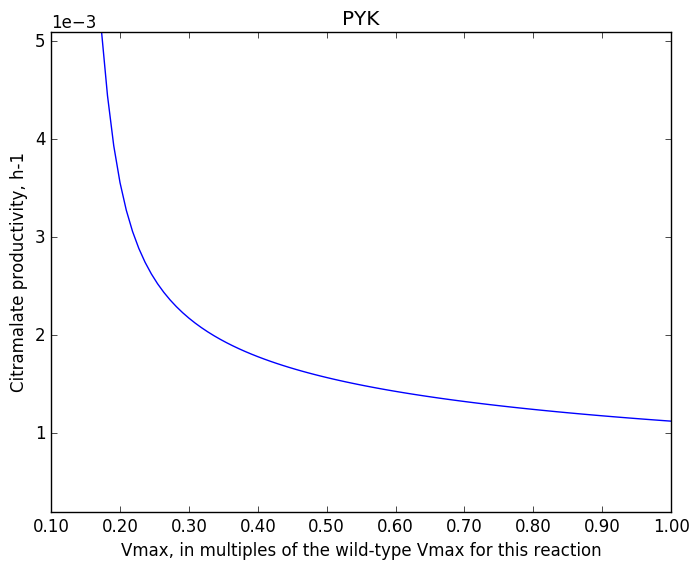
\includegraphics[scale=0.5]{onereacsample}
  \caption{Example of a one-reaction plot: the reaction PYK}
  \label{fig:onereacsample}
\end{figure}

For some enzymes, varying $V_{max}$ values have a greater effect on citramalate productivity than others. I quantified this effect based on the data points of the 0.5 -- 2.0 $V_{max}$ plots\footnote{created early in the project, not included in the final results. I only mention them here because I used information from them in later parts of the project} by taking the difference between the maximum and minimum productivities obtained over the range. Granted, this isn’t the best way to analyse. I’ve tried regression, but it didn’t seem very informative.

This identified CITRA\_SYN, GLT, LPD, GROWTH, ATP\_MAINTENANCE, GDH, ATP\_SYN, ACEA, PYK, and ZWF as among the enzymes that had the greatest effects. Millard \emph{et al}~\cite{millard_metabolic_2017} listed CYTBO, ZWF, GDH, GLT, and GROWTH as the enzymes found to have the largest shares of flux control. They also exert the strongest controls on concentration. These enzymes are followed by LPD, ATP\_MAINTENANCE, ACEA, ATP\_SYN, and PYK

Exchange reactions (XCH\_ACE, XCH\_GLC, and XCH\_P) have no bearing on productivity as all the values in their plots can be attributed to noise. Surprisingly, ACS (acetyl CoA synthetase), ACK (acetate kinase), and PTA (phosphate acetyltransferase), which are all directly related to controlling acetyl CoA levels, do not seem to have ignificant bearings on productivity.

As expected, enzymes found to have the largest shares of flux control create the plots that demonstrate the greatest change in citramalate productivity in response to $V_{max}$ changes. However, CYTBO has a less effect on productivity as would be expected by this explanation. Although PYK does not exert a lot of control over fluxes as expected by its flux control coefficient, it has quite a great effect on citramalate productivity. Possibly it is because the citramalate reaction uses up pyruvate and because PYK is a control point in glycolysis. A few reactions exhibit inflection points in their plots, as shown in table~\ref{tab:inflection}. For reference, the wild-type productivity is 0.001122 h\textsuperscript{-1}. %0.00112225918623

\begin{table}[htbp]
  \caption{Reactions with inflection points}
  \label{tab:inflection}
  \centering
  \begin{tabular}{lrrl}
    Reaction & $V_{max}$ (mM s\textsuperscript{-1}) & Productivity (h\textsuperscript{-1}) & Type\\
    ATP\_syn & 16.804 & 0.00216 & minimum\\
    & 23.724 & 0.00231 & maximum\\
    CITRA\_SYN & 0.545 & 0.01660 & maximum\\
    CYTBO & 5.124 & 0.00113 & maximum\\
    EDA & 0.014 & 0.00112 & maximum\\
    GDH & 4.569 & 0.00149 & maximum\\
    MQO & 1.597 & 0.00098 & minimum\\
    PFK & 0.145 & 0.00113 & maximum
  \end{tabular}
\end{table}

In addition to the list of reactions ordered by effect on citramalate productivity as described earlier, I also extracted a list of reactions arranged by descending order of flux control coefficent (FCC) from the Millard \emph{et al} paper, and used it alongside this list in later parts of the project.

\section{Varying $V_{max}$ values of two reactions at a time}
\label{sec:couples}

Varying $V_{max}$ values of two reactions at a time aimed to identify pairs of reactions that have significant effects on citramalate productivity, which could be used to identify conditions that optimise citramalate productivity. Ideally, one should look at all pairs from the 49 reactions that have $V_{max}$ as a parameter. However, there are such 1,176 pairs, and extrapolating from my experience, it would take about nine hours to run the simulations needed to generate the data points using the conditions used in the project. Furthermore, for most reactions, the change in citramalate productivity was minimal when $V_{max}$ varied over the range of 0.1--10.0 $V_{max}$, so generating such a number of datasets would produce a large amount of useless information.

Therefore, I used only the eight reactions from the top of the list I prepared in section~\ref{sec:onereac}, namely:  CITRA\_SYN, GLT, LPD, ATP\_MAINTENANCE, GDH, ATP\_syn, ACEA, and ZWF. I varied their $V_{max}$ values within 0.1--1.0 $V_{max}$ or 0.1--10.0 $V_{max}$, and plotted the resulting citramalate productivities on 28 heatmaps. The $V_{max}$ values took 10 values in their ranges, so each heatmap had 100 data points. The horizontal axis indicates the absolute $V_{max}$ value of the first reaction in mM s\textsuperscript{-1} and the vertical axis represents the second reaction. So that the numbers that are easily visualised are displayed at each data point, I multiplied the citramalate productivity in h\textsuperscript{-1} by 10,000, as the wild-type productivity is 0.001122. Figure~\ref{fig:heatmapsample} is an example of a heatmap. Here, when the $V_{max}$ of GLT is 256.76 mM s\textsuperscript{-1} and the $V_{max}$ of ACEA is 1.83 mM s\textsuperscript{-1}, productivity is 0.00848.

I also used the reactions with the 10 greatest flux control coefficients to generate heatmaps. The trends seen in most heatmaps suggest simple additive effects, and the heatmaps do not have any additional local maxima or minima, suggesting orthogonality.

\begin{figure}[htbp]
  \centering
  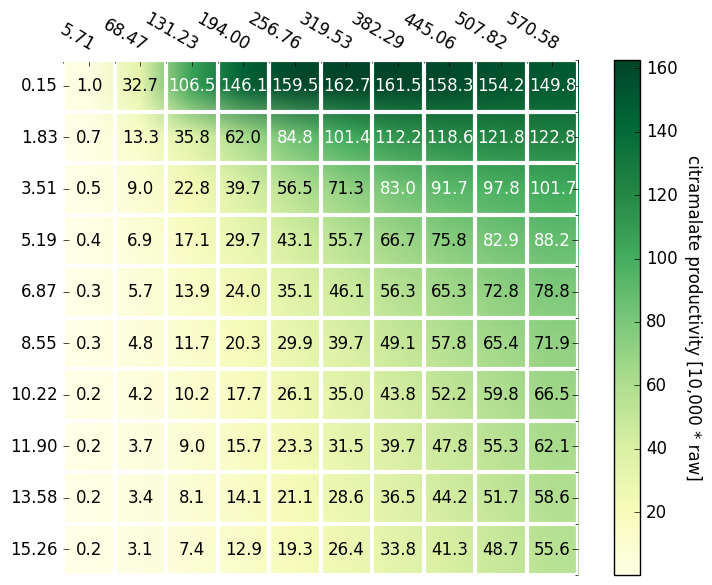
\includegraphics[scale=0.5]{heatmapsample}
  \caption{Example of a heatmap: GLT vs ACEA}
  \label{fig:heatmapsample}
\end{figure}

Plots that involve ATP\_MAINTENANCE exhibit strange behaviour, more evident in higher-resolution heatmaps like figure~\ref{fig:atpmaintenanceheatmap}. The source of this behaviour is unexpected behaviour shown between 0.20 and 0.25 $V_{max}$ in ATP\_MAINTENANCE's one-reaction plot (figure~\ref{fig:atpmaintenanceonereac}). Jorge suggests that it’s because the model is not equipped to deal with small values of $V_{max}$.

\begin{figure}[htbp]
  \centering
  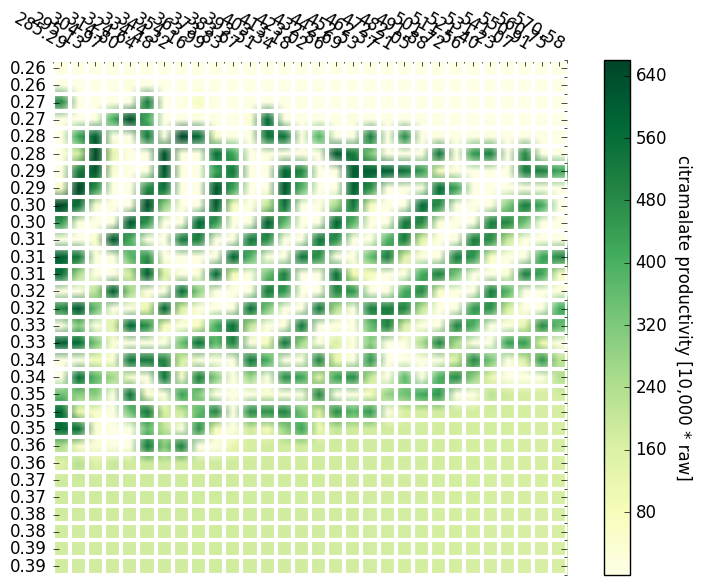
\includegraphics[scale=0.5]{atpmaintenanceheatmap}
  \caption{High-resolution heatmap of GLT vs ATP\_MAINTENANCE}
  \label{fig:atpmaintenanceheatmap}
\end{figure}

\begin{figure}[htbp]
  \centering
  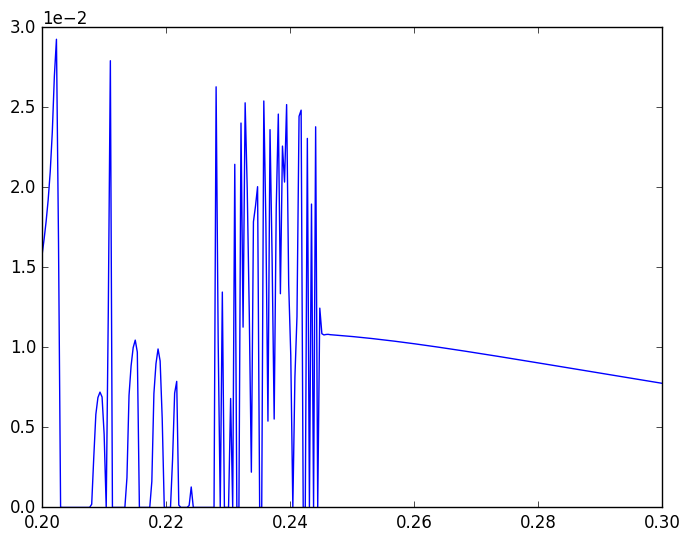
\includegraphics[scale=0.5]{atpmaintenanceonereac}
  \caption{One-reaction plot for ATP\_MAINTENANCE, 300 data points}
  \label{fig:atpmaintenanceonereac}
\end{figure}

\subsection{Verifying that the system has reached steady-state}
\label{ssec:steadystate}

The results are only valid if the system has reached steady state. Steady state is achieved if at the end of simulation time, the greatest rate of change of concentration among the species in the system is less than a small threshold value. In other words:

\[
  \max_{X_{i}} \left | \frac{\mathrm{d}[X_{i}]}{\mathrm{d}t} \right | < \epsilon
\]

where X represents a chemical species, and $\epsilon$ is the threshold value. The threshold value was intially set at \num{1.0e-8}, but then adjusted to \num{1.0e-6} following inspection of heatmaps. For ease of visualisation, I generated heatmaps as I did earlier, but with data points replaced by -1 if the system does not reach steady state in those particular situations (see figure~\ref{fig:steadystate})

\begin{figure}[htbp]
  \centering
  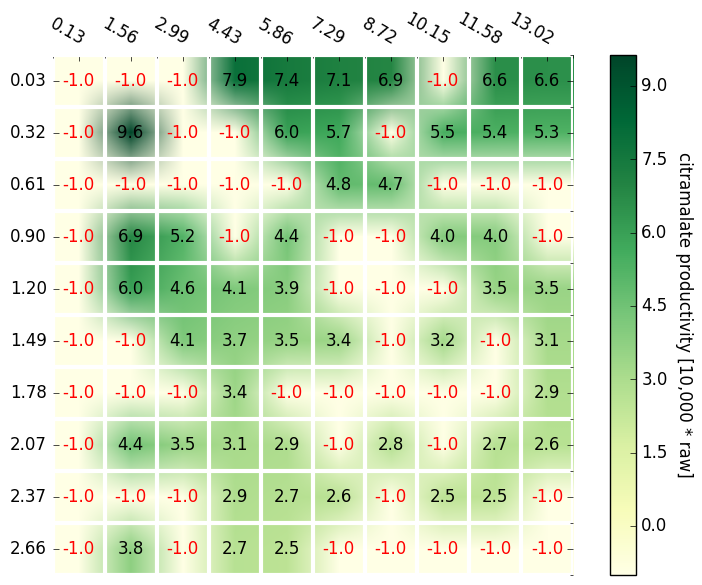
\includegraphics[scale=0.5]{steadystate}
  \caption{Heatmap for ATP\_MAINTENANCE vs ZWF, with threshold set to \num{1.0e-8}}
  \label{fig:steadystate}
\end{figure}

% Make this a paragraph?
I noticed that:
\begin{itemize}
  \item ATP, ADP, P, and Hout are among the species that break the \num{1.0e-8} threshold. However, they stay at around \num{1.0e-7}.
  \item ATP\_MAINTENANCE at 0.1 $V_{max}$ produced rates on the order of \num{e-1}, and ATP\_syn at 0.1 $V_{max}$ produced rates on the order of \num{e-2}. With these two reactions, the species responsible are BPG and OAA
  \item GDH at 0.1 $V_{max}$ produced rates on the order of \num{e-3}, with GLCx and GLCp responsible. This is the only situation where GLCx and GLCp concentrations do not reach steady state.
\end{itemize}

\subsection{Synergistic effects}
\label{ssec:synergistic}

It was difficult to determine if there are synergistic effects between reactions. I began by investigating reactions adjacent to each other. No special effects were observed for PGI and PFK, and a slight synergistic effect was observed for GPM and ENO. Between FBA and GDH, FBA exerts too little effect for the results to be conclusive. In contrast, ACEA and ACEB exhibit \emph{antagonistic} effects, and LPD and GDH, a pair of enzymes far apart from each other in the network seem to have a synergistic effect. My investigations are in the appendix. %insert reference here

\section{Using differential evolution}
\label{sec:de}

% Find way to cite Mier
Differential evolution is a genetic algorithm developed by Storn and Price~\cite{storn_differential_1997}. I used the \texttt{rand/1/bin} strategy, adapting code by Pablo R. Mier (\url{https://pablormier.github.io/2017/09/05/a-tutorial-on-differential-evolution-with-python/}). I used the algorithm to maximise the citramalate productivity while multiple enzymes in a list are varied in their $V_{max}$ values simultaneously.

Differential evolution has the following parameters: $F$, the mutation constant or differential weight; $CR$, the recombination constant or crossover probability, $NP$, the population size; and $D$, the number of dimensions and the number of enzymes investigated simultaneously. The number of iterations is also specified.

Using default values of the parameters, in identifying the $V_{max}$ values of pairs of reactions that resulted in maximal productivity, differential evolution agrees with heatmaps. Occasionally, it discovers maxima not seen in the heatmaps, owing to the relatively low resolution of the heatmaps.

\subsection{Finding optimal parameters}
\label{ssec:deoptimise}

I tested how well the optimal differential evolution parameter values quoted by Storn and Price (1997)~\cite{storn_differential_1997} and Pedersen (2010)~\cite{pedersen_good_2010} optimised citramalate productivity. I used enzymes in the glycolytic pathway (refer to subsection~\vref{ssec:glycolytic}) and enzymes in the list I made in chapter~\vref{sec:onereac}. Values were chosen based on algorithm run time and how fast convergence is realised. They are presented in table~\vref{tab:deoptimise}.

\begin{table}[htbp]
  \caption{Differential evolution optimal parameter search}
  \label{tab:deoptimise}
  \centering
  \begin{tabularx}{\linewidth}{LLLLLLL}
    $F$ & $CR$ & $NP$ & iterations & $D$ & Source\\
    0.8 & 0.7 & 20 & & 2-3 & Mier\\
    0.8 & 0.7 & 20 & 25-40 & 5 & Mier\\
    0.6 & 0.9 & \textless 40 & \textgreater 20 & 5 & Storn\\
    0.6301 & 0.7122 & 17 & 50 & 6-7 & Pedersen (D = 5)\\
    0.6301 & 0.7122 & 17 & 70 & 7 & Pedersen (D = 5)\\
    0.6607 & 0.9426 & 28 & 50 & 7-10 & Pedersen (D = 10, first set), best\\
    0.6702 & 0.2368 & 12 & 100 & 7 & Pedersen (D = 10, second set)\\
  \end{tabularx}
\end{table}

% This subsection may be moved to the appendix or disappear altogether. It's kind of a side-project, and does not really contribute much to the report. Furthermore, this contributes nothing to the methods.
\subsection{Glycolytic enzymes}
\label{ssec:glycolytic}

Originally I used differential evolution with the set of glycolytic enzymes PGI, PFK, FBA, GDH, PGK, GPM, ENO, PYK, and PDH to investigate whether the $V_{max}$ values of all enzymes in a pathway have to be increased to obtain an appreciable increase in the overall flux through the pathway, resulting in higher productivity. Niederberger \emph{et al}~\cite{niederberger_strategy_1992} stated in their paper that flux through all enzymes in a linear pathway must be increased for flux through the pathway to be increased, judging by their experiments on the tryptophan synthesis pathway in yeast. However, Yamamoto \emph{et al}~\cite{yamamoto_overexpression_2012} stated otherwise, and showed that appreciable increases resulted after increasing the flux through only one or two enzymes. My results support the latter.

The objective changed to investigating how much adding an enzyme as an additional dimension in the differential evolution algorithm affects productivity. Adding enzymes relatively low on the section~\ref{sec:onereac} list does not affect the optimum $V_{max}$ values already on there much, and does not cause large improvements in productivity.

%insert appropriate reference to memory leak later
%also make language more formal
This is good because it does not seem necessary to include all enzymes in a pathway in differential evolution, which is a good solution for the memory leak in \texttt{roadrunner}. Additionally, the `curse of dimensionality' results in exponential increases in the time required to return solutions as reactions are added. So it was worth finding out with enzymes had the most effects on productivity after all.

\subsection{Optimisation of citramalate production}
\label{ssec:optcitra}

Using the best parameters found in subsection~\ref{ssec:deoptimise} -- $F$ = 0.6607, $CR$ = 0.9426, $NP$ = 28, and 50 iterations -- with the set of seven reactions CITRA\_SYN, GLT, LPD, GDH, ATP\_syn, ACEA, and ZWF, varying $V_{max}$ values over 0.1--10.0 $V_{max}$ yields optimal $V_{max}$ values as shown in table~\ref{tab:optcitra7} and the corresponding productivity of \num{353.66e-4} h\textsuperscript{-1}. I confirmed that differential evolution was useful by obtaining $V_{max}$ values expected to generate the greatest productivity as expected from one-reaction plots alone and changed the $V_{max}$ values of the seven reactions in the SBML model accordingly. The resulting productivity was computed to be \num{226.96e-4} h\textsuperscript{-1}, lower than the value obtained from differential evolution, thus comfirming the usefulness of the algorithm.

\begin{table}[htbp]
  \caption{Optimisation of citramalate production using seven reactions}
  \label{tab:optcitra7}
  \centering
  \begin{tabular}{lSl}
    Reaction & \multicolumn{1}{c}{Optimal $V_{max}$} & Remark\\
    CITRA\_SYN & 0.4382 & \\
    GLT & 5.706 & 0.1 $V_{max}$ \\
    LPD & 0.006844 & 0.1 $V_{max}$ \\
    GDH & 3.591 & \\
    ATP\_syn & 10.87 & 0.1 $V_{max}$ \\
    ACEA & 0.1526 & 0.1 $V_{max}$ \\
    ZWF & 0.02658 & 0.1 $V_{max}$
  \end{tabular}
\end{table}

Furthermore, I tried the same parameters on 10 enzymes -- CITRA\_SYN, GLT, LPD, GDH, ATP\_syn, ACEA, PYK, ZWF, NDHII, and MQO -- and achieved the productivity of \num{405.5e-4} h\textsuperscript{-1} with a certain set of $V_{max}$ values as shown in table~\ref{tab:optcitra10}. However, 10 reactions exhibited less convergence, as expected by the limitations of the differential evolution algorithm.

\begin{table}[htbp]
  \caption{Optimisation of citramalate production using ten reactions}
  \label{tab:optcitra10}
  \centering
  \begin{tabular}{lSl}
    Reaction & \multicolumn{1}{c}{$V_{max}$ in best solution} & Range\\
    CITRA\_SYN & 1.689 & \\
    GLT & 17.35 & 0.1 $V_{max}$ \\
    LPD & 0.007174 & $\approx$ 0.006844 \\
    GDH & 0.8910 & 0.08666 $\sim$ 0.08910\\
    ATP\_syn & 10.87 & 10.87 $\sim$ 13.01 \\
    ACEA & 0.1826 & 0.1529 $\sim$ 0.01826 \\
    PYK & 0.007472 & $\approx$ 0.007472 \\
    ZWF & 0.02658 & always 0.02658 \\
    NDHII & 10.45 & \\
    MQO & 0.4623 & almost always 0.4623
  \end{tabular}
\end{table}

In parallel, I repeated the investigation using the ten enzymes with the greatest flux control coefficients -- CYTBO, MQO, MDH, ZWF, GLT, GDH, ATP\_syn, ACK, ACEA, and EDD, with results shown in table~\ref{tab:optfcc10}. The productivity was \num{224.2e-4} h\textsuperscript{-1}.

\begin{table}[htbp]
  \caption{Optimisation of citramalate production using ten reactions with the greatest FCCs}
  \label{tab:optfcc10}
  \centering
  \begin{tabular}{lSl}
    Reaction & \multicolumn{1}{c}{Optimal $V_{max}$}\\
    CYTBO & 3.416 \\
    MQO & 1.849 \\
    MDH & 61.15 \\
    ZWF & 0.1072 \\
    GLT & 378.7 \\
    GDH & 4.485 \\
    ATP\_syn & 43.49 \\
    ACK & 20.15 \\
    ACEA & 0.6189 \\
    EDD & 0.6605
  \end{tabular}
\end{table}

Using all 41 biologically relevant reactions that have $V_{max}$ as a parameter does not exhibit enough convergence due to the high number of dimensions, but was able to return productivity on the order of \num{200e-4}, which is still a significant improvement from the wild-type productivity.

\chapter{Enriching the stoichiometric model}
\label{ch:stoich}

% check if FBA is actually linear programming or is actually something more complicated
The stoichiometric model contains flux bounds -- lower and upper bounds -- for each reaction in the model. These bounds can be specified in order to provide constraints for flux balance analysis (FBA)\footnote{Orth \emph{et al}~\cite{orth_what_2010} wrote a very good introduction.}. Using linear programming, FBA aims to find an optimal solution for an objective function, such as the flux through the citramalate synthesis reaction, subject to constraints to the possible flux values. In doing so, the objective function can either be minimised or maximised, and this can be specified when using \texttt{cobra}. The lowest and highest possible values of fluxes through each reaction in the kinetic model provides reasonable bounds for the stoichiometric model.

It should be noted that in the kinetic model, fluxes are in mM s\textsuperscript{-1}, while it is mmol g\textsubscript{DW}\textsuperscript{-1} h\textsuperscript{-1} in the stoichiometric model. Using the cell volume of \num{1.77e-3} L g\textsubscript{DW}\textsuperscript{-1} as specified in the kinetic model, I’ve worked out that converting the units from the kinetic model to the stoichiometric model involves multiplying by 6.372. Because the stoichiometric model does not have any information about enzyme kinetics, the values associated with the kinetic model (with kinetic model units) can be used with the structure of the stoichiometric network without any adjustments.

\section{Creating boundaries for FBA}
\label{sec:bounds}

I varied the $V_{max}$ values of the 49 reactions with $V_{max}$ as a parameter in the kinetic model (with the citramalate synthesis reaction added) in order to find the the lowest and highest possible values of the fluxes through the 69 reactions in the model. Ideally, one should vary all the reactions at once, but in the interest of saving computational time, I first varied $V_{max}$ values of one reaction at a time. I did so over the range of 0.1-10.0 $V_{max}$.

Then, I varied the $V_{max}$ values of many enzymes at a time using differential evolution, obtaining minimum and maximum values of flux. I used a method similar to that used in section~\ref{sec:couples} to obtain the minimum values, specifying the flux through each of the 69 reactions in the kinetic model as the objective function in place of citramalate productivity. Obtaining the maximum values was a matter of adding a minus sign to the objective function in the scripts.

First, I included the eight\footnote{excluding ATP\_MAINTENANCE, see section~\ref{sec:couples}} reactions with the greatest flux control coefficients: CYTBO, MQO, MDH, ZWF, GLT, GDH, ATP\_syn, and ACK. The differential evolution parameters used were $F$ = 0.6607, $CR$ = 0.9426, $NP$ = 28, and 5 iterations~\cite{pedersen_good_2010}. I used the $V_{max}$ range of of 0.3--10.0 $V_{max}$ as using $V_{max}$ values less than 0.3 $V_{max}$ tended to produce run time errors while the \texttt{roadrunner} simulation was run, involving convergence test failures occurring too many times.\footnote{\texttt{RuntimeError: CVODE Error: CV\_CONV\_FAILURE: Convergence test failures occurred too many times (= MXNCF = 10) during one internal timestep or occurred with \textbar{}h\textbar{} = hmin.; In virtual double rr::CVODEIntegrator::integrate(double, double)}}. Judging by the behaviour of ATP\_MAINTENANCE, as described in section~\ref{sec:couples}, results are likely unreliable with small $V_{max}$ values, justifying the use of the more restricted range.

I then moved on to the list of all biologically relevant reactions in the kinetic model, 41 reactions in total. I used the differential evolution parameters of $F$ = 0.6876, $CR$ = 0.9784, $NP$ = 48~\cite{pedersen_good_2010}, and five iterations. To avoid convergence test failures, I set the $V_{max}$ range to 0.5--10.0 $V_{max}$ in this case.

%move this bit? With the mapping section below this the structure is confusing
Bounds generated by including 41 reactions as described above were mostly wider than both bounds generated by including 8 reactions and bounds generated by varying one reaction at a time. In a set of bounds constructed from choosing the best bounds from the three sets described eariler, 43 out of 57 lower bounds and 42 out of 57 lower bounds for reactions in the stoichiometric model with equivalents in the kinetic model were from the bounds generated by including 41 reactions.

\section{Mapping reactions in the kinetic model to the stoichiometric model}
\label{sec:mapping}

Previously, an Anargyros who worked in this group produced a mapping table which mapped reactions in the kinetic model to corresponding reactions in the stoichiometric model. His focus was more on mapping and he did not put specific constraints when generating the bounds, and the method by which he generated these values was not documented. I updated the mapping spreadsheet, correcting mistakes and mapping more enzymes.

To correct Anargyros's mistakes, I changed mapping pairs as follows:

\begin{tabularx}{\linewidth}{|L|L|L|}
  \hline
  Before & After & Notes\\
  \hline
  Kinetic MDH : Stoich. MDH2 & Kinetic MDH : Stoich. MDH, and the reactions are reversed with respect to each other. & Corrected confusion between types of malate dehydrogenases. Re-mapping judged from EC numbers and substrates used\\
  \hline
  Kinetic XCH\_GLC : Stoich. GLCtexi & Kinetic XCH\_GLC : Stoich. GLCtex & Chose a reversible reaction to replace an irreversible one\\
  \hline
  Kinetic XCH\_ACE2 : Stoich. ACACtex & Kinetic XCH\_ACE2 : Stoich. ACtex & Corrected a mistake -- it's acetate exchange, not acetoacetate exchange\\
  \hline
\end{tabularx}

Because reactions in the stoichiometric model are not identical to their kinetic counterparts, I used specific rules to reconcile differences. Stoichiometric model reactions that are identical, only differ by having small chemical species like like \ce{H^+} and \ce{H2O}, only differ by having \ce{CO2} instead of \ce{HCO3^-}, or are indicated as irreversible while its equivalent is reversible in the kinetic model have the same lower and upper bounds. For stoichiometric model reactions that are reversed with respect to their kinetic model counterparts, the values obtained from the kinetic model are negated -- i.e. $(lb, ub) \rightarrow (-ub, -lb)$. Glucose uptake reactions (PTS\_0, PTS\_1, PTS\_2, PTS\_3, PTS\_4) and the pentose pathway reactions X5P\_GAP\_TKT, F6P\_E4P\_TKT, S7P\_R5P\_TKT, F6P\_GAP\_TAL, and S7P\_E4P\_TAL each form different sub-network structures in the stoichiometric model compared to the kinetic model, and therefore do not allow one-to-one mapping. While Anargyros provided limited information for these reactions, after investigating the relationship between flux values in both models by conducting simulations, I devised the following solution, which is applied in newmapper.ods.

\begin{itemize}
\item Forced the flux of Stoich.\ TALA to be equal to the flux of Kinetic S7P\_R5P\_TKT.
\item Forced the flux of Stoich.\ TKT1 and Stoich.\ TKT2 to be equal to half of the flux of Kinetic RPE.
\item Forced the flux of Stoich.\ GLCptspp to be equal to the flux of Stoich.\ GLCtex.
\end{itemize}

These derive from observations that these relationships between flux values hold regardless of the initial conditions.

\section{Flux balance analysis}
\label{sec:fba}

Using the mapping rules described in section~\vref{sec:mapping}, I prepared bounds for FBA from the values obtained in section~\ref{sec:bounds}. Setting the objective to maximising to flux through the citramalate flux reaction, I obtained the results in table~\ref{tab:citramalatefluxresults}.

\begin{table}
  \caption{FBA results using citramalate flux as the objective function}
  \label{tab:citramalatefluxresults}
  \centering
  \begin{tabular}{lS}
    Bounds & Solution\\
    Default & 12.4122\\
    Anargyros's & 0.3067\\
    Varying one reaction at a time & 0.2599\\
    Differential evolution with 8 reactions & 0.1925\\
    Differential evolution with 41 reactions & 0.2922
  \end{tabular}
\end{table}

Then, I looped through all 2,585 reactions in the model and used each as an objective function while using the bounds obtained from including 41 reactions in differential evolution. I set the script to evaluate solutions while setting the objective to both maximising and minimising flux. I used the solutions (optimal minmum and optimal maximum values) as an additional set of bounds for another round of FBA, which returned the solution of 0.2922.

% Merge this section with mapping??
\section{Investigating glucose uptake}
\label{sec:glucoseuptake}

For reference, table~\vref{tab:glucoseuptake} is a mapping between the relevant reactions that I settled on.

\begin{table}
  \caption{Mapping glucose uptake reactions}
  \label{tab:glucoseuptake}
  \centering
  \begin{tabularx}{\linewidth}{LLL}
    Kinetic model & Stoichiometric model & What it is\\
    GLC\_feed & EX\_glc\_(e) & Glucose feed into the environment, set as 0.23 mM s\textsuperscript{-1} in the kinetic model\\
    XCH\_GLC & GLCtex & Glucose transport from the environment into the periplasm\\
    PTS\_0, PTS\_1, PTS\_2, PTS\_3, PTS\_4 & GLCptspp & Glucose uptake from the periplam into the cytoplasm\\
  \end{tabularx}
\end{table}

First, I looked at the relationship between the glucose feed and the fluxes through the other reactions in the kinetic model. The fluxes through XCH\_GLC and the PTS\_X reactions are always the same. XCH\_GLC is equal to GLC\_feed from GLC\_feed = 0 to GLC\_feed = 0.68, after which XCH\_GLC never increases above 0.68 (saturation).

With increasing GLC\_feed, GLCx and GLCp concentrations remain very low until GLC\_feed = 0.68, after which they increase linearly as GLC\_feed increases. The concentration of G6P increases linearly until GLC\_feed = 0.68, at which it immediately plateaus at 3.19

\section{Using information from the Lund medium}
\label{sec:lund}

The patent WO 2015/022496~\cite{eastham_process_2015} (p.79) describes a medium, referred in this project as the Lund medium, for E. coli BW25113 $\Delta$pflB$\Delta$ldhA transformed with pBAD24-cimA fermentation for the optimal production of (R)-citramalic acid:

\begin{tabular}{lSl}
  Glucose & 11.9 & g L\textsuperscript{-1}\\
  \ce{(NH4)2SO4} & 2 & g L\textsuperscript{-1}\\
  \ce{K2HPO4} & 14.6 & g L\textsuperscript{-1}\\
  \ce{NaH2PO4.2H2O} & 3.6 & g L\textsuperscript{-1}\\
  \ce{(NH4)2H} citrate & 0.5 & g L\textsuperscript{-1}\\
  \ce{MgSO4} & 0.24 & g L\textsuperscript{-1}\\
  \ce{CaCl2.2H2O} & 2 & mg L\textsuperscript{-1}\\
  \ce{FeCl3} & 20.06 & mg L\textsuperscript{-1}\\
  \ce{ZnSO4.7H2O} & 0.36 & mg L\textsuperscript{-1}\\
  \ce{CuSO4.5H2O} & 0.32 & mg L\textsuperscript{-1}\\
  \ce{MnSO4.H2O} & 0.30 & mg L\textsuperscript{-1}\\
  \ce{CoCl2.6H2O} & 0.36 & mg L\textsuperscript{-1}\\
  \ce{Na2EDTA.2H2O} & 44.6 & mg L\textsuperscript{-1}
\end{tabular}

Per litre, each chemical species is present in the following amounts (mmol):

\begin{tabular}{lS}
  glucose & 66.05\\
  \ce{NH4^+} & 34.69\\
  \ce{SO4^{2-}} & 17.13\\
  \ce{K^{+}} & 167.6\\
  \ce{Hcitrate} & 2.211\\
  \ce{Mg^{2+}} & 1.994\\
  \ce{Ca^{2+}} & 0.006802\\
  \ce{Cl^-} & 0.3876\\
  \ce{Fe^{3+}} & 0.1237\\
  \ce{Zn^{2+}} & 0.001252\\
  \ce{Cu^{2+}} & 0.001282\\
  \ce{Mn^{2}+} & 0.001775\\
  \ce{Co^{2}+} & 0.001513\\
  EDTA & 0.1198\\
  \ce{Na^+} & 23.32\\
  phosphates & 106.9
\end{tabular}

To conform to the exchange reactions defined in the stoichiometric model, \ce{HPO4^{2-}} and \ce{H2PO4^-} were merged into a `phosphates' species.

I then specifed the maximum rate of exchange of these species into the \emph{E. coli} system by specifying lower bounds for exchange reactions in the stoichiometric model. Exchange reactions for all the above species are present in the stoichiometric model, except for EDTA. I fixed the bound for glucose exchange to -0.23, -0.68, and -10.0 and fixed the bound for the other reactions so that the ratios between the chemical species are conserved. These bounds were added to the boundaries found in section~\ref{sec:bounds} in which 41 enzymes were included in differential evolution.

Only the glucose and citrate exchange reactions have non-zero flux values in the optimal solution. When the exchange reactions for the chemical species present in the Lund model were unbouded, glucose exchange is -11.13 and citrate exchange is -1.20.

Given
\begin{itemize}
\item a concentration of a chemical species $[X_{i}]$
\item the growth rate or dilution rate $\mu$
\item a measured OD\textsubscript{600}
\item that a OD\textsubscript{600} of 1 corresponds to an \emph{E. coli} concentration of $Z$, expressed in g\textsubscript L\textsuperscript{-1} (0.36--0.39 in the literature) %citation here
\end{itemize}
  
the exchange rate $R$ for that chemical species can be calculated as follows:

\[
  R = \frac{\mu[X_{i}]}{OD_{600} \cdot Z}
\]

\chapter{Remarks}
\label{ch:remarks}

In this project, I was able to identify reactions in the kinetic model that had relatively large effects on citramalate productivity, and used these reactions to inform the processes of investigating the effects of pairs of reactions and using differential evolution to optimise citramalate productivity. Steady-state conditions were realised in most combinations of $V_{max}$ values used in the project, and situations in which steady-state conditions were not realised can be attributed to certain reactions acquiring low $V_{max}$ values. I showed that the kinetic model is not reliable with such low values of $V_{max}$. Furthermore, I demonstrated than differential evolution is a viable method in finding the best $V_{max}$ values to optimise citramalate productivity, and that only including a small proportion of the reactions in the kinetic model is sufficient.

I created an improved method of mapping reactions in the kinetic model to corresponding reactions in the stoichiometric model and assigning bounds for FBA. I also demonstrated that differential evolution can be used to generate useful FBA bounds. Finally, I investigated how the concentrations of chemical species in the Lund medium can be used to set bounds for the exchange reactions in the stoichiometric model.

\section{Issues in the project}
\label{sec:issues}

The most consequential issue within this project is that \texttt{roadrunner} has a memory leak in \texttt{roadrunner.RoadRunner()}. Memory can only be relased when the Python program ends. The function is required to run the simulations required to generate almost all the data in the project. \texttt{libsbml.writeSBMLToString()} also makes a contribution. This function writes a modified SBML file, namely with different $V_{max}$ values, derived from a model object in the program, to a string stored in the memory accessible by the Python program. \texttt{roadrunner.RoadRunner()} then takes the string as an argument in creating an object which can be used to run simulations. Arguably, it is more logical to pass the model object directly into the simulation, but as of 17 August 2018, the official documentation for \texttt{libroadrunner} 1.5.1 states that `In future version, we will also support loading directly from a \texttt{libSBML} Document object.'

The memory leak has a large impact on the project as almost all scripts include running simulations on modified kinetic models many times in succession. The workaround of writing shell scripts to run and stop the scripts after each round of looping which includes running simulations partially alleviates the problem. This method, however, does not work with differential evolution on account of how the algorithm was built in. As a result, the number of iterations that can be carried out before Python uses up all the random access memory in the system is limited, and adequate convergence may not be realised when there are many dimensions ($D$ is high). The `curse of dimensionality', a limitation of differential evolution, exacerbates the problem: with an increasing number of dimensions, the difficulty of finding the optimal solution increases exponentially.

Alternatives to the differential evolution algorithm used in the project exist in the \texttt{scipy} and \texttt{pygmo} modules. These alternatives can used strategies other than \texttt{rand/1/bin} and can carry out self-optimisation of parameters. Furthermore, they can perform dithering on $F$, which has been shown to improve convergence~\cite{storn_differential_1997}. However, they seem to take longer to compute and even exacerbates the memory leak problem. As they are black-box optimisation methods, I am unable to probe into the problem or improve on the algorithms.

Fortunately, the \texttt{cobra} module used to manipulate the stoichiometric model and FBA does not have such memory leaks.

There was also an issue with preparing a list of a small number of enzymes to be investigated in the heatmaps and differential evolution, in order to save computational time. The method I used to quantify the effect that varying $V_{max}$ of each reaction had on citramalate productivity as described in section~\ref{sec:onereac} had no real statistical basis (it was sort of a quick-and-dirty method). Any method that uses the data points I generated, however, will have to rationalise using a specific range of $V_{max}$ values, as the ranges in use are arbitrary. Using the flux control coefficients was an alternative, and I generated data accordingly, but here the reactions are sorted by how much control they have over the network as a whole, and not by control over the citramalate synthesis reaction.

Additionally, generating one-reaction plots using flux through the citramalate synthesis reaction and growth as objective functions, which are included in the results directories, instead of citramalate productivity called into question the validity of using flux through the citramalate synthesis reaction as a proxy for citramalate productivity in FBA. The shape of the plots of flux through citramalate synthesis differ a lot from that of citramalate productivity, and growth contributes more to the shape of the plots of citramalate productivity. With this in mind, I have investigated using citramalate productivity as the objective function in FBA, but the existing tools in \texttt{cobra} are limited to linear functions. As citramalate productivity is expressed as the product of two functions that exist in the stoichiometric model, other packages such as CPLEX or Gurobi must be used. However, both these are proprietary, though Gurobi offers a free licence for universities.

As for mapping reactions in the kinetic model to the stoichiometric model, I based it on observations from running simulations rather than theoretical knowledge behind the model networks. Therefore, I do not know the validity. However, I observed that switching from Anargyros's limited treatment of the glucose uptake and pentose phosphate pathway reactions to the method I used did not cause a significant change to the optimal citramalate productivity found by FBA.

% move discussion to main section of report? Equations feel more appropriate there
Finally, there were issues with working out appropriate FBA bounds from the chemical composition of the Lund medium, which is the matter of translating the concentration of a chemical species into a flux value for the corresponding exchange reaction. This is mainly due to the lack of definitive OD\textsubscript{600} value for \emph{E. coli} in the stoichiometric model, as Orth \emph{et al.}~\cite{orth_comprehensive_2011} did not specifyit. Complicating the issue, there is a study by Kavvas \emph{et al.}~\cite{kavvas_updated_2018} which included variations of the same stoichiometric model of \emph{Mycobacterium tuberculosis} that had different bounds for exchange reactions according to differing media conditions, but the bounds seem to be arbitrary round numbers and do not reflect the ratios between the concentrations of the chemical species present in the media. Even if appropriate bounds can be worked out, the observations seen from when the exchange reactions were unbounded as described in section~\ref{sec:lund} calls into question how useful they would be.

\section{Future direction and suggestions}
\label{sec:future}

Building up on this project may go down some of the following avenues:

\begin{itemize}
\item Use a simulator apart from \texttt{roadrunner} that does not have a memory leak
\item Use standard deviations to quantify the effect that varying $V_{max}$ values of reach reaction in the kinetic model has on citramalate productivity
\item Develop a method to investigate whether there are synergistic effects between reactions
\item Investigate alternatives to \texttt{scipy} and \texttt{pygmo} in implementing a differential evolution algorithm, and investigating optimal parameter searches
\item Use other genetic algorithms apart from differential evolution
\item Generate boundaries for FBA using more iterations in differential evolution
\item Investigate the theoretical basis behind mapping between the kinetic and stoichiometric models
\end{itemize}
  
\section{Notes about files}
\label{sec:files}

The files included alongside this report include text files, image files, spreadsheets, and Python scripts. The text files mainly contain information about the models, such as wild-type conditions, and results from various parts of the project. The image files include the one-reaction plots and heatmaps. Important spreadsheets include an improved version of Anargyros's mapping spreadsheet and one to convert the minimum and maximum fluxes in the kinetic model to corresponding fluxes to be applied in FBA. Finally, the Python scripts were written to manipulate the two models, generate the images, and generate the data in the project.

These files are in a version-controlled directory and in a \emph{private} GitHub repository owned by \url{https://github.com/arinwongprommoon/}, which only I have access to.

\appendix
\chapter*{Appendix}
\addcontentsline{toc}{chapter}{Appendix}
\renewcommand{\thesection}{\Alph{section}}

\section{Reactions in the kinetic model}
\label{ap:kineticreactionlist}

This is a list of the 68 reactions in the kinetic model with their wild-type $V_{max}$ values as specified in the SBML file. 49 reactions have $V_{max}$ as a parameter.

\begin{longtable}{lS}
  \toprule
  Reaction & \multicolumn{1}{c}{Wild-type $V_{max}$ (mM s\textsuperscript{-1})}\\
  \midrule
  ACEA & 1.52595\\
ACEB & 0.352769\\
ACEK\_1 & \multicolumn{1}{c}{None}\\
ACEK\_2 & \multicolumn{1}{c}{None}\\
ACK & 7.23\\
ACN\_1 & 9.72413\\
ACN\_2 & 9.86571\\
ACS & 7.3\\
ADK & \multicolumn{1}{c}{None}\\
ATP\_MAINTENANCE & 1.30166\\
ATP\_syn & 108.733\\
CYA & \multicolumn{1}{c}{None}\\
CYTBO & 8.54045\\
DOS & \multicolumn{1}{c}{None}\\
EDA & 0.0775241\\
EDD & 0.111359\\
ENO & 11.7189\\
F6P\_E4P\_TKT & \multicolumn{1}{c}{None}\\
F6P\_GAP\_TAL & \multicolumn{1}{c}{None}\\
FBA & 21.6978\\
FBP & 0.215583\\
FUMA & 53.3414\\
GDH & 8.66573\\
GL6P\_HYDROLYSIS & \multicolumn{1}{c}{None}\\
GLC\_feed & \multicolumn{1}{c}{None}\\
GLT & 57.0584\\
GND & 4.08105\\
GPM & 10.9934\\
GROWTH & 9.74137\\
ICD & \multicolumn{1}{c}{None}\\
LPD & 0.0684413\\
MAD & 6.64269\\
MDH & 6.11492\\
MQO & 4.62283\\
NADH\_req & 23.0735\\
NDHII & 30.8306\\
PCK & 8.08777\\
PDH & 961.706\\
PFK & 0.185253\\
PGI & 2.32456\\
PGK & 16.1089\\
PGL & 11.5967\\
PIT & 7.146\\
PNT\_req & \multicolumn{1}{c}{None}\\
PPC & 21.439\\
PPS & 0.0163772\\
PTA & 2.7\\
PTS\_0 & \multicolumn{1}{c}{None}\\
PTS\_1 & \multicolumn{1}{c}{None}\\
PTS\_2 & \multicolumn{1}{c}{None}\\
PTS\_3 & \multicolumn{1}{c}{None}\\
PTS\_4 & \multicolumn{1}{c}{None}\\
PYK & 0.74716\\
RPE & 6.00103\\
RPI & 8.0\\
S7P\_E4P\_TAL & \multicolumn{1}{c}{None}\\
S7P\_R5P\_TKT & \multicolumn{1}{c}{None}\\
SDH & 1.56184\\
SK & 76.8163\\
SQR & 3.41617\\
TPI & 24.1843\\
X5P\_GAP\_TKT & \multicolumn{1}{c}{None}\\
XCH\_ACE1 & 100.0\\
XCH\_ACE2 & 100.0\\
XCH\_GLC & 100.0\\
XCH\_P & 100.0\\
ZWF & 0.2658\\
\_ACE\_OUT & \multicolumn{1}{c}{None}\\
\bottomrule
\end{longtable}

Of these, 41 correspond to real enzymes in \emph{E. coli}: ACEA, ACEB, ACK, ACN\_1, ACN\_2, ACS, ATP\_syn, CITRA\_SYN, CYTBO, EDA, EDD, ENO, FBA, FBP, FUMA, GDH, GLT, GND, GPM, LPD, MAD, MDH, MQO, PCK, PDH, PFK, PGI, PGK, PGL, PIT, PPC, PPS, PTA, PYK, RPE, RPI, SDH, SK, SQR, TPI, and ZWF.

\section{One-reaction list}
\label{ap:onereactionlist}

Here is the list of kinetic model reactions ordered by effect on citramalate productivity, as quantified by the method described in section~\ref{sec:onereac}. This list is termed the `one-reaction list' in this report.
\begin{longtable}{lS}
  \toprule
  Reaction & \multicolumn{1}{c}{Difference}\\
  \midrule
CITRA\_SYN & 0.0047592827\\
GLT & 0.0028143645\\
LPD & 0.0024355991\\
GROWTH & 0.0015196535\\
ATP\_MAINTENANCE & 0.0013313081\\
GDH & 0.0009114522\\
ATP\_syn & 0.0007611072\\
ACEA & 0.0007511846\\
PYK & 0.0007372515\\
ZWF & 0.0003202479\\
NDHII & 0.0002585753\\
MQO & 0.0002267894\\
NADH\_req & 0.0002253453\\
MDH & 0.0002253183\\
MAD & 0.000194721\\
PGI & 0.0001198466\\
PCK & 0.0001030438\\
PPC & 9.98662735514203E-05\\
ACEB & 7.90308554654898E-05\\
PDH & 7.25091053451472E-05\\
ENO & 0.000052497\\
CYTBO & 4.01304504630247E-05\\
PFK & 0.000029278\\
SDH & 2.34810929815527E-05\\
GPM & 0.000017908\\
RPI & 1.57468888476676E-05\\
RPE & 1.17187158724425E-05\\
GND & 7.7970772124512E-06\\
FBA & 5.78669223682236E-06\\
PIT & 4.2598627200143E-06\\
XCH\_GLC & 2.30450409889268E-06\\
EDD & 1.45414534944354E-06\\
TPI & 1.13784049543585E-06\\
ACK & 5.9384816856003E-07\\
SQR & 2.76393130356403E-07\\
ACN\_1 & 0.000000163\\
ACN\_2 & 1.34302723317709E-07\\
PGL & 1.18091121640955E-07\\
EDA & 1.13285023008386E-07\\
FBP & 6.4369739164339E-08\\
PTA & 0.000000059\\
PPS & 3.50591144481546E-08\\
FUMA & 1.57341325584745E-08\\
PGK & 1.23830399983461E-08\\
ACS & 3.41921927208243E-09\\
SK & 2.53497706831883E-09\\
XCH\_ACE1 & 3.6139094993469E-10\\
XCH\_P & 1.30011316599662E-10\\
XCH\_ACE2 & 1.15399255906298E-10\\
\bottomrule
\end{longtable}

\section{Synergistic effects between reactions in the kinetic model}
\label{ap:synergistic}

\section{Glycolytic enzymes and differential evolution}
\label{ap:glycolytic}

\printbibliography

\end{document}
